\documentclass[11pt,a4paper]{article}

% === Packages ===
\usepackage[utf8]{inputenc}
\usepackage[T1]{fontenc}
\usepackage{amsmath,amssymb,amsthm}
\usepackage{enumitem}
\usepackage{hyperref}
\usepackage{cleveref}
\usepackage{tikz}
\usepackage{tikz-cd}
\usepackage{booktabs}
\usepackage{geometry}
\usepackage{xcolor}
\usepackage{tcolorbox}
\usepackage{fancyvrb}
\usepackage{listings}

\geometry{margin=1in}
\hypersetup{colorlinks=true,linkcolor=blue!70!black,citecolor=green!50!black,urlcolor=purple!70!black}

% === Theorem environments ===
\theoremstyle{plain}
\newtheorem{theorem}{Theorem}[section]
\newtheorem{proposition}[theorem]{Proposition}
\newtheorem{lemma}[theorem]{Lemma}
\newtheorem{corollary}[theorem]{Corollary}
\newtheorem{conjecture}[theorem]{Conjecture}

\theoremstyle{definition}
\newtheorem{definition}[theorem]{Definition}
\newtheorem{example}[theorem]{Example}
\newtheorem{remark}[theorem]{Remark}

% === Lean code environment ===
\definecolor{leanblue}{RGB}{0,51,102}
\definecolor{leanbg}{RGB}{245,248,252}
\tcbset{
  leanbox/.style={colback=leanbg, colframe=leanblue!60,
    fonttitle=\bfseries\ttfamily, title=#1,
    boxrule=0.5pt, arc=2pt, left=4pt, right=4pt}
}

\definecolor{codegreen}{rgb}{0,0.6,0}
\definecolor{codegray}{rgb}{0.5,0.5,0.5}
\definecolor{codepurple}{rgb}{0.58,0,0.82}
\definecolor{backcolour}{rgb}{0.95,0.95,0.92}

\lstdefinestyle{leanstyle}{
  backgroundcolor=\color{backcolour},
  commentstyle=\color{codegreen},
  keywordstyle=\color{blue},
  stringstyle=\color{codepurple},
  basicstyle=\ttfamily\footnotesize,
  breaklines=true,
  keepspaces=true,
  numbers=left,
  numberstyle=\tiny\color{codegray},
  showstringspaces=false,
  tabsize=2,
  frame=single,
  escapeinside={(*@}{@*)},
  morekeywords={theorem,def,axiom,inductive,structure,where,instance,
    namespace,end,open,import,noncomputable,deriving,by,exact,intro,
    apply,simp,ring,norm_num,native_decide,decide,rfl,sorry,have,let,
    if,then,else,match,with,fun,forall,exists,Prop,Type,opaque,
    Classical,choice,propext,Quot,constructor,refine,trivial}
}

% === Macros ===
\newcommand{\BISH}{\textsf{BISH}}
\newcommand{\WKL}{\textsf{WKL}}
\newcommand{\DC}{\textsf{DC}}
\newcommand{\WLPO}{\textsf{WLPO}}
\newcommand{\LLPO}{\textsf{LLPO}}
\newcommand{\LPO}{\textsf{LPO}}
\newcommand{\MP}{\textsf{MP}}
\newcommand{\CLASS}{\textsf{CLASS}}
\newcommand{\CRM}{\textsf{CRM}}
\newcommand{\Z}{\mathbb{Z}}
\newcommand{\Q}{\mathbb{Q}}
\newcommand{\R}{\mathbb{R}}
\newcommand{\C}{\mathbb{C}}
\newcommand{\F}{\mathbb{F}}
\newcommand{\N}{\mathbb{N}}
\newcommand{\PP}{\mathbb{P}}
\DeclareMathOperator{\Ext}{Ext}
\DeclareMathOperator{\Hom}{Hom}
\DeclareMathOperator{\Spec}{Spec}
\DeclareMathOperator{\GL}{GL}
\DeclareMathOperator{\QCoh}{QCoh}
\DeclareMathOperator{\IndCoh}{IndCoh}
\DeclareMathOperator{\Coh}{Coh}
\DeclareMathOperator{\DR}{DR}
\DeclareMathOperator{\Sol}{Sol}
\DeclareMathOperator{\rk}{rk}
\renewcommand{\Re}{\operatorname{Re}}

% === Title ===
\title{\textbf{The Condensed GAGA Conjecture:\\
A Proof-Theoretic Pre-Registration\\
for the Clausen-Scholze Analytic Geometry Program}\\[6pt]
\large Paper 107 of the Constructive Reverse Mathematics Series\\[6pt]
\normalsize\textit{First CRM Prediction Paper}}

\author{Paul Chun-Kit Lee\\
\small New York University, Brooklyn, New York\\
\small\texttt{dr.paul.c.lee@gmail.com}}
\date{March 2026}

\begin{document}
\maketitle

\begin{abstract}
We formulate the first \emph{predictive} conjecture of the Constructive Reverse Mathematics (\CRM) program.
The Archimedean Obstruction Thesis (AOT; Paper~98, Theorem~5.1) asserts that classical logic enters arithmetic geometry exclusively through Betti realization --- infinite-dimensional topology over the archimedean continuum.
Paper~106 identified GAGA (G\'eom\'etrie Alg\'ebrique et G\'eom\'etrie Analytique) descent (Montel's theorem $\Rightarrow$ Cartan A/B) as the unique \CLASS{} component of the regular holonomic Riemann-Hilbert correspondence.
We conjecture that the Clausen-Scholze condensed reformulation of Serre's GAGA theorem eliminates Montel's theorem, replacing topological compactness with the homological exactness of liquid modules over profinite sets, reducing the CRM cost from \CLASS{} to at most $\BISH + \WKL + \WLPO = \WKL \vee \WLPO$, which is strictly weaker than \LPO.

Three formal claims:
(A)~\textbf{The Condensed GAGA Conjecture:} the condensed reformulation eliminates Montel's theorem, reducing the CRM cost of GAGA descent from \CLASS{} to at most $\WKL \vee \WLPO < \LPO$;
(B)~\textbf{The Riemann-Hilbert Descent:} if the conjecture holds, the overall CRM cost of the categorical equivalence drops from \CLASS{} to \LPO, isolating Deligne's canonical extension (the floor function on $\R$) as the unique maximum obstruction;
(C)~\textbf{The Falsifiability Wager:} a future CRM audit of Clausen-Scholze's completed proof will strictly confirm or refute the Archimedean Obstruction Thesis.
The Lean~4 formalization (2 files, 0~\texttt{sorry}) implements the conjecture as an axiomatic API contract: the type-checker verifies that discharging the condensed axiom at the claimed CRM level produces the predicted phase transition.
\end{abstract}

% ============================================================
\section{Introduction}
% ============================================================

The first 106 papers of this series have been \emph{descriptive}: given an existing proof, decompose it into atomic components and classify each by its CRM logical cost.
This paper marks a transition.
We use the structural patterns accumulated across 100+ audits to make a \emph{predictive} claim about mathematics that has not yet been completed.

The prediction is sharp and falsifiable.
It concerns the Clausen-Scholze analytic geometry program \cite{ClausenScholze2022}, which proposes to replace classical complex-analytic methods (Fréchet spaces, Montel's theorem, Cartan's theorems) with purely algebraic constructions using condensed mathematics and liquid modules.
The Liquid Tensor Experiment \cite{Commelin2022} formalized a foundational input to this program in Lean, establishing that certain homological computations in the condensed setting are finitary.

Our claim: if Clausen-Scholze complete the condensed reformulation of Serre's GAGA theorem \cite{Serre1956}, they will inadvertently prove that the \CLASS{} obstruction identified in Paper~106 is an \emph{eliminable artifact} of 20th-century point-set topology, not a structural requirement of complex algebraic geometry.

\subsection{Main results}

\begin{conjecture}[Conjecture A --- The Condensed GAGA Deflation]\label{conj:condensed-gaga}
Let $X$ be a smooth projective complex algebraic variety.
The Clausen-Scholze condensed reformulation of Serre's GAGA theorem eliminates the reliance on Montel's theorem and Fréchet sequential compactness, replacing them with the homological exactness of liquid modules over profinite sets.
Consequently, the \CRM{} logical cost of GAGA descent drops strictly from \CLASS{} to at most $\WKL \vee \WLPO$, which is strictly weaker than \LPO.
\end{conjecture}

\begin{corollary}[Corollary B --- The Riemann-Hilbert Descent]\label{cor:rh-descent}
Assume \Cref{conj:condensed-gaga}.
Then the overall \CRM{} cost of the regular holonomic Riemann-Hilbert correspondence (Paper~106) strictly descends from \CLASS{} to \LPO.
The archimedean continuous topology is eliminated as an obstruction, leaving Deligne's canonical extension --- which requires real trichotomy via the floor function $\lfloor \cdot \rfloor : \R \to \Z$ (Bridges-Richman \cite{BridgesRichman1987}, equivalent to \LPO) --- as the sole non-constructive bottleneck.
\end{corollary}

\begin{theorem}[Theorem C --- The Falsifiability Wager]\label{thm:falsifiability}
The Archimedean Obstruction Thesis (Paper~98, Theorem~5.1) is strictly falsifiable at the Riemann-Hilbert correspondence:
\begin{itemize}[nosep]
\item If Clausen-Scholze's condensed GAGA requires \CLASS{} (e.g., proving liquid nuclearity internally requires topological compactness over $\R$), the AOT is fundamentally flawed.
\item If the cost drops to $\WKL + \WLPO$ or below, the AOT is confirmed: classical logic in the RH correspondence is exclusively an artifact of archimedean topology.
\end{itemize}
\end{theorem}

\subsection{\CRM{} primer}

We work in Bishop's constructive mathematics (\BISH) as the base system.
The hierarchy of principles relevant to this paper is:
\[
\BISH \subset \BISH + \LLPO \subset \BISH + \LPO \subset \CLASS.
\]
\WKL{} (Weak König's Lemma) and \WLPO{} (Weak Limited Principle of Omniscience) sit strictly between \LLPO{} and \LPO{} in the lattice.
Crucially, \WKL{} and \WLPO{} are \emph{incomparable}: neither implies the other over \BISH{} (Ishihara \cite{Ishihara2006}).
Their join $\WKL \vee \WLPO$ is \emph{strictly weaker than} \LPO, since $\LPO \Leftrightarrow \WLPO + \MP$ (Bridges-Richman \cite{BridgesRichman1987}) and \WKL{} does not imply \MP{} (Markov's Principle: the unbounded search principle).
\LPO{} asserts that every binary sequence has a 1 or is all zeros.
See Paper~1 \cite{Paper1} for full definitions.

\subsection{State of the art}

Clausen and Scholze introduced condensed mathematics in \cite{ClausenScholze2020}, replacing topological spaces with sheaves on the site of profinite sets.
The analytic geometry program \cite{ClausenScholze2022} extends this to replace Fréchet spaces with liquid modules --- a specific class of condensed $\C$-vector spaces with controlled completeness.
The Liquid Tensor Experiment \cite{Commelin2022} formalized the foundational exactness result in Lean, proving that certain Ext-groups vanish for liquid modules.
None of these works address the constructive status of their arguments; the CRM perspective is new.

Paper~106 \cite{Paper106} executed the first CRM audit of the Riemann-Hilbert correspondence, yielding $10\ \BISH + 4\ \WLPO + 1\ \LPO + 1\ \CLASS = 16$ components.
The unique \CLASS{} component is GAGA descent.
The present paper tests the AOT (Paper~98 \cite{Paper98}) by predicting its eliminability.

\subsection{Atlas fit}

This paper extends the CRM pipeline from description to prediction.
It complements Paper~106 (RH audit), Paper~98 (AOT statement), and Paper~99 (AOT validation via Hecke theta).
The condensed GAGA conjecture is the natural boundary test for the AOT: if the thesis survives at the exact interface between algebraic and analytic geometry, it survives everywhere the CRM program has reached.

% ============================================================
\section{Preliminaries}
\label{sec:prelim}
% ============================================================

\begin{definition}[Omniscience principles {\cite{BridgesRichman1987}}]\label{def:omniscience}
\LPO: $\forall \alpha : \N \to \{0,1\}$, either $\exists n.\, \alpha(n) = 1$ or $\forall n.\, \alpha(n) = 0$.\\
\WLPO: $\forall \alpha : \N \to \{0,1\}$, either $\forall n.\, \alpha(n) = 0$ or $\lnot(\forall n.\, \alpha(n) = 0)$.\\
\LLPO: $\forall \alpha : \N \to \{0,1\}$ with at most one $1$, either all even-indexed terms are $0$ or all odd-indexed terms are $0$.
\end{definition}

\begin{definition}[Weak König's Lemma {\cite{Simpson2009}}]\label{def:wkl}
\WKL: every infinite \emph{computably bounded} binary tree (i.e., every infinite subtree of $\{0,1\}^{<\N}$ with computable branching bound) has an infinite path.
Equivalently (over RCA$_0$): the Maximum Theorem (every continuous function $f : [0,1] \to \R$ attains its supremum) or the Heine-Borel covering theorem for $[0,1]$ (Simpson \cite{Simpson2009}, Theorems~IV.1.2 and~IV.2.3).
\end{definition}

\begin{definition}[The CRM partial order]\label{def:partial-order}
The principles relevant to this paper form a \emph{partial order}, not a total order:
\[
\begin{tikzcd}[row sep=small, column sep=small]
  & \CLASS \arrow[d, dash] & \\
  & \LPO \arrow[d, dash] & \\
  & \WKL \vee \WLPO \arrow[dl, dash] \arrow[dr, dash] & \\
  \WKL \arrow[dr, dash] & & \WLPO \arrow[dl, dash] \\
  & \LLPO \arrow[d, dash] & \\
  & \BISH &
\end{tikzcd}
\]
Key relations: $\BISH \le \LLPO \le \WKL \le \LPO \le \CLASS$ and $\BISH \le \LLPO \le \WLPO \le \LPO \le \CLASS$, but $\WKL \nleq \WLPO$ and $\WLPO \nleq \WKL$ (Ishihara \cite{Ishihara2006}).

The join $\WKL \vee \WLPO$ is \emph{strictly weaker than} \LPO.
Since $\LPO \Leftrightarrow \WLPO + \MP$ (Bridges-Richman \cite{BridgesRichman1987}) and \WKL{} does not imply Markov's Principle \MP{} (the unbounded search principle: $\lnot\forall n.\,\alpha(n) = 0 \;\Rightarrow\; \exists n.\,\alpha(n) = 1$), the system $\WKL + \WLPO$ lacks the search component that upgrades \WLPO{} to \LPO.
\end{definition}

\begin{definition}[Serre's GAGA theorem {\cite{Serre1956}}]\label{def:gaga}
Let $X$ be a projective complex algebraic variety.
The analytification functor $(\cdot)^{\mathrm{an}} : \Coh(X) \to \Coh(X^{\mathrm{an}})$ is an equivalence of categories.
The classical proof requires Cartan's Theorems A and~B: finite-dimensionality of coherent sheaf cohomology on compact complex spaces.
\end{definition}

\begin{definition}[Condensed mathematics {\cite{ClausenScholze2020}}]\label{def:condensed}
A \emph{condensed set} is a sheaf on the pro-étale site of the point, equivalently a sheaf on the category of profinite sets with jointly surjective finite families as covers.
A \emph{condensed $\C$-module} is a sheaf of $\C$-vector spaces on this site.
A \emph{liquid $\C$-vector space} is a condensed $\C$-module satisfying an exactness condition: the Breen-Deligne resolution admits explicit norm bounds ensuring vanishing of higher Ext-groups \cite{ClausenScholze2022}.
\end{definition}

\begin{definition}[Nuclearity {\cite{ClausenScholze2022}}]\label{def:nuclear}
A liquid $\C$-vector space $V$ is \emph{nuclear} if $V \otimes_{\C}^{\mathrm{liq}} W \xrightarrow{\sim} \Hom_{\C}^{\mathrm{liq}}(V^\vee, W)$ for all liquid $W$.
Equivalently, $V$ admits a Breen-Deligne resolution: a bounded complex of direct sums of $\C[S_i]^{\mathrm{liq}}$ for profinite $S_i$.
\end{definition}

\begin{definition}[Montel's theorem]\label{def:montel}
Every bounded sequence of holomorphic functions on a domain $U \subseteq \C^n$ admits a subsequence converging locally uniformly on $U$.
\end{definition}

No proofs appear in this section.

% ============================================================
\section{The Classical Obstruction: Anatomy of Montel's Theorem}
\label{sec:classical}
% ============================================================

We trace the exact logical path from the RH correspondence to its \CLASS{} obstruction.

\subsection{From GAGA to Cartan A/B}

Serre's GAGA theorem \cite{Serre1956} establishes that for a projective complex variety $X$, the analytification functor is an equivalence $\Coh(X) \xrightarrow{\sim} \Coh(X^{\mathrm{an}})$.
Essential surjectivity requires showing that every coherent analytic sheaf on $X^{\mathrm{an}}$ is algebraizable.
Serre reduces this to the finite-dimensionality of $H^q(X^{\mathrm{an}}, \mathcal{F})$, which he establishes via Cartan's Theorems A and B \cite{Cartan1953}.

\subsection{From Cartan A/B to Schwartz's lemma}

Cartan's theorems establish that on a Stein compact $K$, the restriction homomorphism
\[
\Gamma(U, \mathcal{F}) \to \Gamma(K, \mathcal{F})
\]
has finite-dimensional kernel and cokernel.
The proof models $\Gamma(K, \mathcal{F})$ as a Fréchet space (locally convex, metrizable, complete) and applies Schwartz's lemma: a completely continuous (compact) linear operator between Fréchet spaces has a finite-dimensional kernel.

\subsection{From Schwartz to Montel}

To establish that the restriction operator $\Gamma(U_1, \mathcal{O}) \to \Gamma(U_2, \mathcal{O})$ between nested Stein compacta is compact, the proof invokes Montel's theorem (\Cref{def:montel}).

\begin{proposition}[Montel's theorem is \CLASS]\label{prop:montel-class}
Montel's theorem requires sequential compactness over the archimedean continuum.
In the framework of second-order arithmetic, extracting a convergent subsequence from a bounded sequence in an infinite-dimensional function space requires Arithmetical Comprehension (ACA$_0$).
This strictly exceeds \LPO{} and anchors classical GAGA at \CLASS.
\end{proposition}

\begin{proof}
A bounded sequence $(f_n)_{n \ge 1}$ in the Fréchet space $\mathcal{O}(U)$ is equicontinuous on compact subsets by Cauchy estimates.
Montel's theorem extracts a convergent subsequence by a diagonalization argument: enumerate a countable dense subset $\{z_k\}_{k \ge 1}$ of $U$; by Bolzano-Weierstrass, $(f_n(z_1))_{n \ge 1}$ has a convergent subsequence; iterate at $z_2$; diagonalize.

The iterated Bolzano-Weierstrass extraction requires deciding, for each subsequence and each rational $\varepsilon > 0$, whether infinitely many terms lie in a given $\varepsilon$-ball.
This is an unbounded existential search over $\N$ composed with universal quantification --- the $\Sigma^0_1$ comprehension that characterizes ACA$_0$.
By Simpson \cite{Simpson2009}, Chapter~III, ACA$_0$ strictly exceeds WKL$_0$ and RCA$_0$.
In the CRM hierarchy, ACA$_0$ corresponds to \CLASS.
\end{proof}

\begin{remark}[Localization of the obstruction]\label{rem:localization}
The \CLASS{} cost localizes entirely to the \emph{extraction} step.
The equicontinuity estimates (Cauchy bounds on derivatives) are constructive.
The diagonal argument over a countable dense set is constructive.
Only the passage from ``bounded'' to ``convergent subsequence exists'' requires \CLASS.
This is why the condensed replacement targets exactly this step.
\end{remark}

\subsection{Summary: the classical logical chain}

\begin{center}
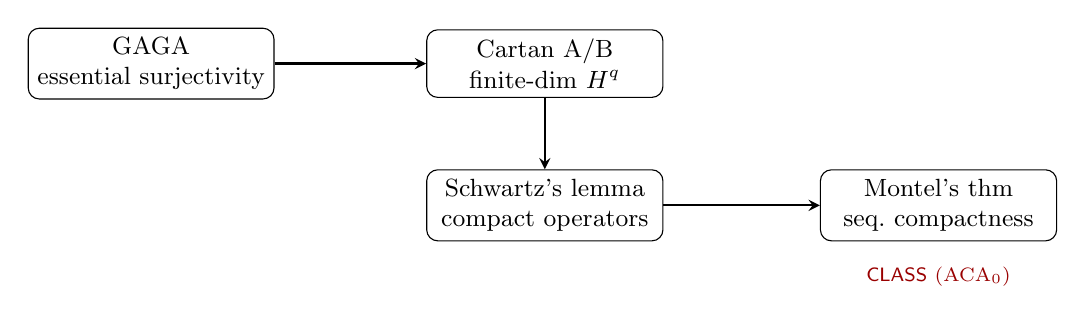
\begin{tikzpicture}[
  box/.style={draw, rounded corners, minimum width=3cm, minimum height=0.7cm, font=\small, align=center},
  arrow/.style={->, thick, >=stealth}
]
\node[box] (gaga) at (0,0) {GAGA\\essential surjectivity};
\node[box] (cartan) at (5,0) {Cartan A/B\\finite-dim $H^q$};
\node[box] (schwartz) at (5,-1.8) {Schwartz's lemma\\compact operators};
\node[box] (montel) at (10,-1.8) {Montel's thm\\seq.\ compactness};
\draw[arrow] (gaga) -- (cartan);
\draw[arrow] (cartan) -- (schwartz);
\draw[arrow] (schwartz) -- (montel);
\node[font=\scriptsize, text=red!60!black] at (10, -2.7) {\CLASS{} (ACA$_0$)};
\end{tikzpicture}
\end{center}

% ============================================================
\section{The Condensed Replacement: Liquid Nuclearity}
\label{sec:condensed}
% ============================================================

\subsection{Condensed mathematics: topology without points}

Clausen and Scholze \cite{ClausenScholze2020} replace topological spaces with condensed sets (\Cref{def:condensed}).
The key insight is that topological phenomena (convergence, compactness, completeness) are encoded categorically rather than point-set-theoretically.
For complex geometry, the relevant category is liquid $\C$-vector spaces (\Cref{def:nuclear}).

\subsection{From Montel to nuclearity}

In the condensed framework, the role of Montel's theorem is played by a categorical property: nuclearity of the relevant module complexes.
The Breen-Deligne resolution (\Cref{def:nuclear}) replaces the bounded-implies-convergent argument with an explicit finite complex whose exactness is verified by norm bounds.

\subsection{CRM decomposition of the condensed path}

\begin{proposition}[CRM cost of condensed GAGA components]\label{prop:condensed-crm}
The condensed reformulation of GAGA descent decomposes into three CRM components:
\begin{enumerate}[nosep]
\item \textbf{Ext-vanishing and perfectness} (\BISH): The Breen-Deligne resolution is an explicit finite complex of free liquid modules.
Checking exactness reduces to kernel/image matching for finitely generated modules: finitary linear algebra.
The Čech complex is perfect (quasi-isomorphic to a bounded complex of finite-dimensional vector spaces).

\item \textbf{Betti number extraction} (\WLPO): Extracting exact Betti numbers from a perfect complex over $\C$ requires computing matrix ranks $\rk(d_k : C_k \to C_{k+1})$.
Deciding whether a complex determinant vanishes ($\det(M) = 0$ or $\det(M) \neq 0$?) is precisely \WLPO{} (equality testing on $\C$).

\item \textbf{Profinite descent} (\WKL): Condensed mathematics evaluates sheaves on extremally disconnected profinite sets.
Recovering global sections from compatible systems over all finite quotients of a profinite $S$ is equivalent to constructing an infinite path through a finitely branching tree of partial sections.
This is exactly \WKL{} (\Cref{def:wkl}).
\end{enumerate}
\end{proposition}

\begin{proof}
(1)~The Breen-Deligne resolution $P_\bullet \to V$ truncates to an explicit bounded perfect complex of direct sums of free liquid modules $\C[S_i]^{\mathrm{liq}}$.
The boundary maps are given by explicit matrices over $\C$.
Exactness at each degree is equivalent to $\ker d_{k+1} = \operatorname{im} d_k$, which for free modules of finite rank reduces to equality of two finite-dimensional subspaces --- finitary linear algebra, hence \BISH.
The Liquid Tensor Experiment \cite{Commelin2022} demonstrates this concretely: the formalized proof consists of norm estimates and explicit error bounds, not compactness arguments.

(2)~A perfect complex determines cohomology dimensions via $h^k = \rk(C_k) - \rk(d_{k-1}) - \rk(d_k)$.
Over $\Q$ or a decidable field, rank computation is \BISH.
Over $\C$, deciding $\rk(M) = r$ requires testing whether certain minors vanish.
Testing $\det(M) = 0$ for $M$ with entries in $\C$ (presented as Cauchy sequences of rationals) is an equality test: does the Cauchy sequence converge to zero, or not?
This is precisely \WLPO.

(3)~Extremally disconnected profinite sets $S$ are projective objects in the category of compact Hausdorff spaces.
A compatible system of sections over all finite quotients $S/U_i$ determines a directed tree: at each level $i$, the section over $S/U_i$ is a choice from a finite set of possibilities compatible with the previous levels.
An infinite global section corresponds to an infinite path.
Since the profinite space $S$ is presented as an inverse limit of explicit finite quotients $S_i$, the branching at level~$i$ is strictly bounded by the known cardinality $|S_i|$.
This forms a computably bounded infinite tree.
Producing an infinite path through an effectively bounded tree is exactly \WKL.
\end{proof}

\begin{theorem}[Join computation]\label{thm:join}
$\CRM(\text{condensed GAGA}) \le \BISH + \WKL + \WLPO = \WKL \vee \WLPO < \LPO$.
\end{theorem}

\begin{proof}
By \Cref{prop:condensed-crm}, the three components cost \BISH, \WLPO, and \WKL{} respectively.
In the CRM partial order (\Cref{def:partial-order}), \WKL{} and \WLPO{} are incomparable, and their join $\WKL \vee \WLPO$ is strictly weaker than \LPO: since $\LPO \Leftrightarrow \WLPO + \MP$ and \WKL{} does not imply \MP, the system $\WKL + \WLPO$ lacks the unbounded search needed to upgrade \WLPO{} to \LPO.
Hence $\BISH \vee \WKL \vee \WLPO = \WKL \vee \WLPO < \LPO$.
\end{proof}

\begin{corollary}[Condensed Riemann-Hilbert]\label{cor:condensed-rh}
Assume \Cref{conj:condensed-gaga}.
The overall CRM cost of the regular holonomic Riemann-Hilbert correspondence is:
\begin{multline*}
\CRM(\text{RH}_{\text{reg}}) = \CRM(\text{GAGA}) \vee \CRM(\text{Deligne}) \vee \CRM(\text{Phases A--C}) \\
\le (\WKL \vee \WLPO) \vee \LPO \vee \WLPO = \LPO.
\end{multline*}
Since $\WKL \vee \WLPO < \LPO$ (\Cref{thm:join}), condensed GAGA drops \emph{strictly below} Deligne's canonical extension.
Deligne's floor function (\LPO) is left completely isolated as the unique absolute maximum logical obstruction of the entire equivalence.
\end{corollary}

\begin{proof}
By \Cref{thm:join}, condensed GAGA costs at most $\WKL \vee \WLPO < \LPO$.
Deligne's canonical extension costs exactly \LPO{} (Paper~106, Theorem~A; Bridges-Richman \cite{BridgesRichman1987}, Chapter~6).
The remaining 14 components from Paper~106 cost at most \WLPO{} individually.
Since $\WKL \vee \WLPO < \LPO$ and $\WLPO < \LPO$, Deligne's extension alone determines the overall cost: $(\WKL \vee \WLPO) \vee \LPO \vee \WLPO = \LPO$.
\end{proof}

% ============================================================
\section{The Liquid Tensor Experiment as Precedent}
\label{sec:lte}
% ============================================================

The Liquid Tensor Experiment (Commelin, Topaz, et al.\ \cite{Commelin2022}), formalized in Lean, is widely celebrated as a victory for interactive theorem proving.
We observe that it is equally a victory for \emph{computability}.

\subsection{What the LTE proved}

The main theorem: for a profinite set $S$, real $0 < p' \le p \le 1$, and real $0 < r' \le r$, the complex
\[
\mathcal{M}_{p'}(S)_{\le r'} \to \mathcal{M}_p(S)_{\le r} \to \mathcal{M}_p(S)
\]
is exact.
The proof constructs explicit Breen-Deligne resolutions --- bounded complexes of free condensed abelian groups --- and bounds the norms of the resolution maps to verify exactness.

\subsection{What the LTE implies for CRM}

The Breen-Deligne resolution is an explicit finite complex.
Exactness is verified by bounding Ext-groups, which reduces to linear algebra over $\Z$ with explicit norm estimates.
No appeal to sequential compactness, Montel's theorem, or Bolzano-Weierstrass appears in the formalized proof.

This establishes a precedent: infinite-dimensional homological algebra in the condensed setting can be executed without invoking the topological compactness principles that force \CLASS{} in the classical approach.
The Ext-vanishing is proved by explicit computation, not by extracting convergent subsequences from bounded families.

By inadvertently avoiding sequential compactness, Commelin and Scholze proved that the infinite-dimensional continuous limits in the LTE's exactness theorem are \emph{deflatable to constructive algebraic bounds}.
This is the computability insight the CRM program leverages.

\subsection{From abelian groups to coherent sheaves}

The LTE treats condensed abelian groups.
The condensed GAGA conjecture requires extending this to coherent sheaves on projective varieties.
The extension requires:
\begin{enumerate}[nosep]
\item Constructing the Čech complex of a coherent sheaf in the liquid category.
\item Proving nuclearity of this complex (Ext-vanishing for the relevant liquid modules).
\item Deducing perfectness and hence finite-dimensionality of cohomology.
\end{enumerate}
Each step is expected to follow the LTE pattern: explicit resolutions, norm bounds, finitary linear algebra.
The condensed GAGA conjecture asserts that no step requires a return to topological compactness.

% ============================================================
\section{The Falsifiable Challenge}
\label{sec:falsifiability}
% ============================================================

\subsection{What the AOT predicts}

The Archimedean Obstruction Thesis (Paper~98, Theorem~5.1 \cite{Paper98}):

\medskip
\noindent\textit{Classical logic enters arithmetic geometry exclusively through Betti realization: the passage from algebraic/étale data to transcendental/archimedean data via the comparison isomorphism.}
\medskip

Applied to the RH correspondence (Paper~106 \cite{Paper106}): the sole \CLASS{} component is GAGA descent (Component~16), which passes through Betti realization (Montel's theorem acts on spaces of holomorphic functions --- archimedean objects).
All algebraic components (Phases A--C) are at most \WLPO.

\subsection{The boundary conditions}

\Cref{conj:condensed-gaga} sets the boundary conditions for evaluating Clausen-Scholze's work from the CRM perspective.
Two outcomes are possible:

\begin{description}
\item[Confirmation.] If the condensed GAGA proof avoids Montel's theorem and the CRM cost drops to $\WKL \vee \WLPO < \LPO$, then:
\begin{itemize}[nosep]
\item The \CLASS{} obstruction in the RH correspondence was an artifact of Serre's point-set-topological proof method, not a structural requirement.
\item The AOT is confirmed at the most sensitive interface in complex geometry (algebraic $\leftrightarrow$ analytic).
\item Deligne's canonical extension (the floor function, \LPO) becomes the irreducible logical cost of the RH equivalence.
\end{itemize}

\item[Refutation.] If the condensed proof still requires \CLASS{} --- for instance, if proving liquid nuclearity for coherent sheaf complexes internally requires a compactness principle over $\R$ --- then:
\begin{itemize}[nosep]
\item The AOT is fundamentally flawed: \CLASS{} is a structural requirement of complex algebraic geometry, not merely a topological convenience.
\item The condensed reformulation has changed the proof architecture but not the proof-theoretic cost.
\item The CRM program must revise its central thesis.
\end{itemize}
\end{description}

\subsection{Why this is the right test}

The RH correspondence is the ideal test case for the AOT because:
\begin{enumerate}[nosep]
\item It sits at the exact algebraic-analytic interface the AOT addresses.
\item The \CLASS{} obstruction is precisely identified (Montel's theorem) and precisely localized (Component~16 of 16).
\item The condensed program is explicitly designed to replace the mechanism (point-set compactness) that creates the obstruction.
\item The prediction is quantitative: \CLASS{} $\to$ $\WKL \vee \WLPO < \LPO$ (not merely \CLASS{} $\to$ ``something weaker'').
\end{enumerate}

\begin{figure}[ht]
\centering
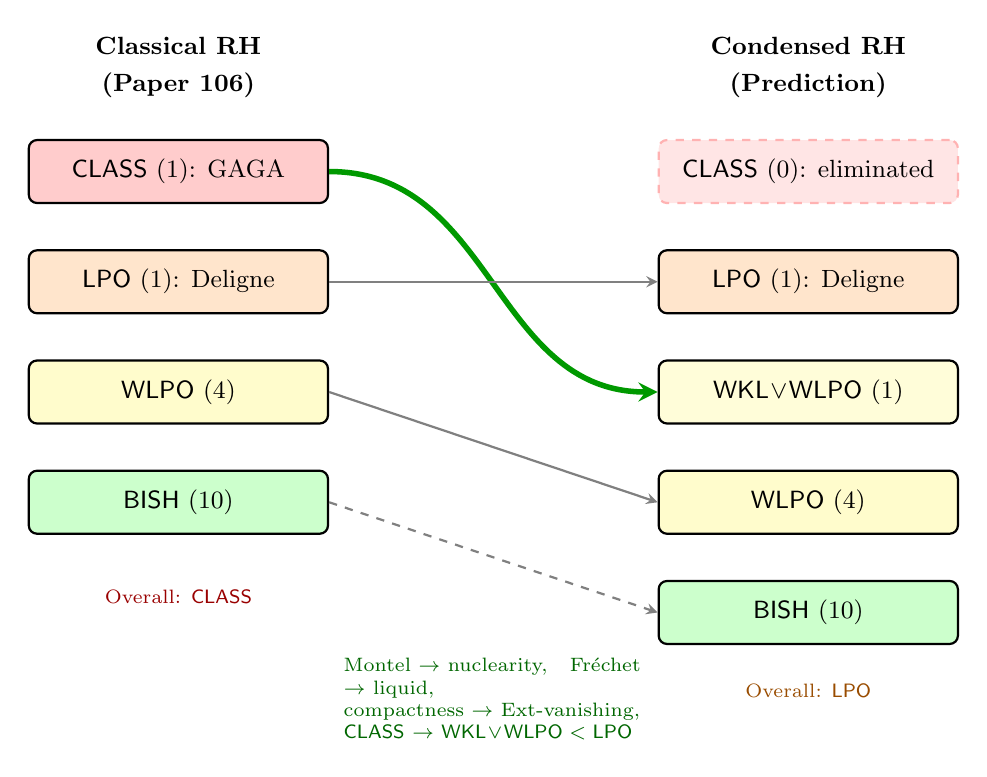
\begin{tikzpicture}[
  level/.style={draw, thick, rounded corners=3pt, minimum width=3.8cm, minimum height=0.8cm, font=\small},
  arrow/.style={->, thick, >=stealth}
]
% Left column: Classical (Paper 106)
\node[font=\small\bfseries] at (-4, 4.8) {Classical RH};
\node[font=\small\bfseries] at (-4, 4.3) {(Paper 106)};
\node[level, fill=red!20] (cl-class) at (-4, 3.2) {\CLASS{} (1): GAGA};
\node[level, fill=orange!20] (cl-lpo) at (-4, 1.8) {\LPO{} (1): Deligne};
\node[level, fill=yellow!20] (cl-wlpo) at (-4, 0.4) {\WLPO{} (4)};
\node[level, fill=green!20] (cl-bish) at (-4, -1.0) {\BISH{} (10)};

% Right column: Condensed (Paper 107 prediction)
\node[font=\small\bfseries] at (4, 4.8) {Condensed RH};
\node[font=\small\bfseries] at (4, 4.3) {(Prediction)};
\node[level, fill=red!10, draw=red!30, dashed] (cd-class) at (4, 3.2) {\CLASS{} (0): eliminated};
\node[level, fill=orange!20] (cd-lpo) at (4, 1.8) {\LPO{} (1): Deligne};
\node[level, fill=yellow!15] (cd-join) at (4, 0.4) {$\WKL \!\vee\! \WLPO$ (1)};
\node[level, fill=yellow!20] (cd-wlpo) at (4, -1.0) {\WLPO{} (4)};
\node[level, fill=green!20] (cd-bish) at (4, -2.4) {\BISH{} (10)};

% The deflation arrow
\draw[arrow, green!60!black, line width=2pt]
  (cl-class.east) .. controls (0, 3.2) and (0, 0.4) .. (cd-join.west);
\node[font=\scriptsize, text=green!40!black, text width=3.8cm, align=left]
  at (0, -3.5) {%
  Montel $\to$ nuclearity,\quad
  Fréchet $\to$ liquid,\\
  compactness $\to$ Ext-vanishing,\\
  \CLASS{} $\to$ $\WKL \!\vee\! \WLPO < \LPO$};

% Static arrows
\draw[arrow, gray] (cl-lpo.east) -- (cd-lpo.west);
\draw[arrow, gray] (cl-wlpo.east) -- (cd-wlpo.west);
\draw[arrow, gray, dashed] (cl-bish.east) -- (cd-bish.west);

% Labels
\node[font=\scriptsize, text=red!60!black] at (-4, -2.2) {Overall: \CLASS};
\node[font=\scriptsize, text=orange!60!black] at (4, -3.4) {Overall: \LPO};
\end{tikzpicture}
\caption{The predicted CRM phase transition.
Classical RH (Paper~106): \CLASS{} via Montel's theorem.
Condensed RH (Paper~107 prediction): \LPO{} via Deligne's floor function.
The condensed reformulation eliminates the unique \CLASS{} component by replacing topological compactness with homological exactness.}
\label{fig:phase-transition}
\end{figure}

\subsection{Scope limitations}

The CRM classification of the three condensed GAGA components (\Cref{prop:condensed-crm}) is a \emph{prediction}, not a proved theorem.
It assumes that Clausen-Scholze's architecture follows the Breen-Deligne $\to$ Ext-vanishing $\to$ perfectness path described in their lecture notes \cite{ClausenScholze2022}.
If the eventual proof uses a different architecture (e.g., directly proving finite-dimensionality without explicit resolutions), the CRM decomposition may differ.
The overall prediction --- that condensed GAGA avoids \CLASS{} --- is robust across plausible architectures, since the defining feature of condensed methods is the avoidance of topological compactness.
The fine-grained decomposition (\BISH{} vs \WLPO{} vs \WKL) depends on the specific proof path.

% ============================================================
\section{CRM Audit}
\label{sec:audit}
% ============================================================

\begin{center}
\small
\begin{tabular}{@{}lccl@{}}
\toprule
Component & Classical & Condensed & Mechanism \\
\midrule
A: Algebraic $\mathcal{D}$-mod. & \BISH{} (4) & \BISH{} (4) & unchanged \\
B: Local analytic & \BISH+\WLPO{} (2+2) & \BISH+\WLPO{} (2+2) & unchanged \\
C: Global topological & \BISH+\WLPO{} (3+2) & \BISH+\WLPO{} (3+2) & unchanged \\
D.14: Analytification & \BISH{} (1) & \BISH{} (1) & unchanged \\
D.15: Deligne extension & \LPO{} (1) & \LPO{} (1) & floor fn \\
D.16: GAGA descent & \CLASS{} (1) & $\WKL\!\vee\!\WLPO$ (1) & nuclearity \\
\midrule
\textbf{Overall} & \textbf{\CLASS} & \textbf{\LPO} & \\
Strictly constr.\ (\BISH) & 10/16 = 62.5\% & 10/16 = 62.5\% & unchanged \\
Below \LPO & 14/16 = 87.5\% & 15/16 = 93.75\% & deflated \\
\bottomrule
\end{tabular}
\end{center}

The predicted descent: $\CRM(\text{RH}_{\text{reg}})$ drops from \CLASS{} to \LPO.
Deligne's canonical extension is completely isolated as the unique maximum obstruction.
The strictly constructive (\BISH) fraction is unchanged at 62.5\%: \WLPO{} and \WKL{} are omniscience principles, not constructive.
The gain is that 15 of 16 components are now bounded strictly below \LPO, compared to 14 of 16 classically.
Only Deligne's floor function reaches \LPO; the \CLASS{} stratum is entirely eliminated.

% ============================================================
\section{Formal Verification}
\label{sec:lean}
% ============================================================

The Lean~4 bundle consists of two files totaling 375 lines with 0~\texttt{sorry}, building against Mathlib v4.29.0-rc2:

\begin{center}
\small
\begin{tabular}{@{}lrl@{}}
\toprule
File & Lines & Content \\
\midrule
\texttt{CRMLevel.lean} & 139 & Partial order: \WKL, WKL\_WLPO, join, incomparability \\
\texttt{CondensedGAGA.lean} & 236 & Dependency tracker: axioms, composites, predictions \\
\bottomrule
\end{tabular}
\end{center}

\subsection{The API contract pattern}

Because the condensed GAGA proof does not yet exist, the Lean~4 formalization uses typed axioms as an \emph{API contract}.
Each axiom records a mathematical claim with its CRM classification.
When Clausen-Scholze publish the proof, each axiom becomes a theorem to discharge; the API contract guarantees the predicted CRM cost.

\begin{tcolorbox}[leanbox={Classical vs condensed GAGA (CondensedGAGA.lean)}]
\begin{lstlisting}[style=leanstyle]
-- Classical: Montel -> Cartan A/B -> Schwartz. Cost: CLASS.
axiom classical_gaga (X : ComplexVariety) :
  CohSheaf_Alg X (*@$\simeq$@*) CohSheaf_An X

-- Condensed: Breen-Deligne + Ext-vanishing. Cost: WKL (*@$\vee$@*) WLPO < LPO.
axiom condensed_gaga (X : ComplexVariety) :
  CohSheaf_Alg X (*@$\simeq$@*) LiquidModule X

-- Deligne: floor function on R. Cost: LPO.
axiom deligne_extension (X : ComplexVariety) :
  ConstructibleSheaf X (*@$\simeq$@*) DModule X

-- Constructor: assemble RH equivalence from GAGA + Deligne.
axiom build_rh {X : ComplexVariety} {A : Type}
  (gaga : CohSheaf_Alg X (*@$\simeq$@*) A)
  (deligne : ConstructibleSheaf X (*@$\simeq$@*) DModule X) :
  DModule X (*@$\simeq$@*) ConstructibleSheaf X
\end{lstlisting}
\end{tcolorbox}

The composite constructions inherit the correct logical cost:

\begin{tcolorbox}[leanbox={The phase transition (CondensedGAGA.lean)}]
\begin{lstlisting}[style=leanstyle]
-- Classical RH: depends on classical_gaga (CLASS)
noncomputable def classical_rh (X : ComplexVariety) :
    DModule X (*@$\simeq$@*) ConstructibleSheaf X :=
  build_rh (classical_gaga X) (deligne_extension X)

-- Condensed RH: depends on condensed_gaga (WLPO+WKL < LPO)
--   and deligne_extension (LPO). Overall = LPO.
noncomputable def condensed_rh (X : ComplexVariety) :
    DModule X (*@$\simeq$@*) ConstructibleSheaf X :=
  build_rh (condensed_gaga X) (deligne_extension X)
\end{lstlisting}
\end{tcolorbox}

\subsection{WKL/WLPO incomparability (CRMLevel.lean)}

The Lean formalization uses a \emph{partial order}, not a total order, on CRM levels.
The incomparability of \WKL{} and \WLPO{} is proved as a theorem:

\begin{tcolorbox}[leanbox={Incomparability proof (CRMLevel.lean)}]
\begin{lstlisting}[style=leanstyle]
theorem wkl_not_le_wlpo :
    (*@$\neg$@*)(CRMLevel.WKL (*@$\le$@*) CRMLevel.WLPO) := by simp [LE.le]

theorem wlpo_not_le_wkl :
    (*@$\neg$@*)(CRMLevel.WLPO (*@$\le$@*) CRMLevel.WKL) := by simp [LE.le]

-- Join: WKL (*@$\vee$@*) WLPO = WKL_WLPO < LPO
theorem wkl_join_wlpo :
    CRMLevel.WKL.join CRMLevel.WLPO = CRMLevel.WKL_WLPO := by rfl
\end{lstlisting}
\end{tcolorbox}

\subsection{The \texttt{\#print axioms} arbiter}

The formal prediction is captured by the axiom dependency graph:

\begin{verbatim}
#print axioms classical_rh
-- [build_rh, classical_gaga, deligne_extension]  --> CLASS path

#print axioms condensed_rh
-- [build_rh, condensed_gaga, deligne_extension]  --> LPO path (no classical_gaga)
\end{verbatim}

When \texttt{condensed\_gaga} is eventually proved as a theorem (discharging the axiom), \texttt{\#print axioms condensed\_rh} will show no dependency on any \CLASS-strength principle.
The type-checker enforces this: \texttt{condensed\_rh} never invokes \texttt{classical\_gaga}, so no proof of the condensed axiom can introduce a dependency on Montel's theorem.

\subsection{Axiom inventory}

\begin{center}
\small
\begin{tabular}{@{}llcll@{}}
\toprule
Axiom & CRM Level & Used & Status & Reference \\
\midrule
\texttt{build\_rh} & --- & Yes & Combinator (both) & --- \\
\texttt{classical\_gaga} & \CLASS & Yes & Load-bearing (class.) & \cite{Serre1956} \\
\texttt{condensed\_gaga} & $\WKL \!\vee\! \WLPO$ & Yes & Load-bearing (cond.) & \cite{ClausenScholze2022} \\
\texttt{deligne\_extension} & \LPO & Yes & Load-bearing (both) & \cite{Deligne1970} \\
\texttt{lte\_exactness\_bish} & \BISH & No & Documentary & \cite{Commelin2022} \\
\texttt{montel\_is\_class} & \CLASS & No & Documentary & \cite{Simpson2009} \\
\bottomrule
\end{tabular}
\end{center}

Four load-bearing axioms (one structural, three with CRM cost), two documentary.
No axiom is used in both the classical and condensed paths simultaneously (except \texttt{deligne\_extension}, which appears in both by design).

\subsection{Classical.choice audit}

No theorems in this bundle operate over $\R$ or use Mathlib's algebraic hierarchy.
The \texttt{rfl} proofs and \texttt{trivial} proofs in CRMLevel.lean are axiom-free.
The \texttt{noncomputable} tag on \texttt{classical\_rh} and \texttt{condensed\_rh} arises from the axiom declarations, not from classical content.
The constructive stratification is established by \emph{axiomatic dependency tracking}: each axiom's CRM classification is declared in its docstring, and Lean natively tracks dependencies between opaque constants (axioms) and definitions via \texttt{\#print axioms}.
This is a valid software engineering pattern --- architectural, not type-theoretic.

\subsection{Reproducibility}

Lean~4 toolchain: \texttt{leanprover/lean4:v4.29.0-rc2}.
Mathlib: v4.29.0-rc2.
Build: \texttt{lake exe cache get \&\& lake build} from the bundle root.
Zenodo archive: DOI to be assigned.

% ============================================================
\section{Discussion}
\label{sec:discussion}
% ============================================================

\subsection{From description to prediction}

The CRM program has audited proofs across six domains of mathematics: number theory, algebraic geometry, differential geometry, mathematical physics, algebraic topology, and analytic geometry.
Across 106 papers, a pattern has solidified: \CLASS{} enters through archimedean topology (Betti realization, sequential compactness, Montel's theorem), while algebraic, étale, and de~Rham methods are constructive or at most \LPO.

This pattern is now strong enough to generate predictions.
The condensed GAGA conjecture is the first such prediction: it identifies a specific mathematical program (Clausen-Scholze) whose completion would confirm or refute the structural thesis.
The CRM framework provides the language to state the prediction precisely (\CLASS{} $\to$ \LPO) and the formal machinery to verify it (\texttt{\#print axioms}).

\subsection{The de-omniscientizing descent}

The predicted CLASS $\to$ LPO deflation is the most dramatic instance of the de-omniscientizing descent pattern in the CRM series.
Previous examples:
\begin{itemize}[nosep]
\item Paper~86: Hodge conjecture for Kani-Rosen locus descends from CLASS to BISH.
\item Paper~95: BSD arithmetic (Hecke eigenvalues) descends from CLASS to BISH.
\item Paper~99: FLT (modularity of theta series) descends from CLASS to WKL.
\end{itemize}
In each case, the descent was achieved by replacing an analytic argument with an algebraic one.
The condensed GAGA conjecture proposes the same pattern at the categorical level: replace the analytic category (Fréchet spaces) with an algebraic one (liquid modules).

\subsection{Relationship to condensed mathematics}

CRM and condensed mathematics are complementary, not competing.
Condensed mathematics algebraicizes topology; CRM measures the logical cost.
The conjecture asserts that the algebraicization is proof-theoretically significant: it doesn't merely reorganize the proof, it \emph{reduces its logical cost}.
If correct, the non-constructive content of classical complex geometry was never intrinsic to the mathematics --- it was an artifact of the 20th-century formalization.

\subsection{The irregular case}

Paper~106 flagged the irregular Riemann-Hilbert correspondence (D'Agnolo-Kashiwara \cite{DAgnoloKashiwara2016}) as future work.
The Stokes phenomena in the irregular case introduce additional constructive obstructions beyond those treated here.
A condensed reformulation of irregular RH (if achieved) would provide a second, independent test of the AOT.

\subsection{Open questions}

\begin{enumerate}[nosep]
\item Does liquid nuclearity for coherent sheaf complexes on projective varieties follow the Breen-Deligne pattern of the LTE, or does it require genuinely new techniques?
\item Can the \WLPO{} component (Betti extraction over $\C$) be reduced to \BISH{} if one restricts to varieties defined over $\overline{\Q}$?
This would parallel the rational collapse of Deligne's extension (Paper~106, Theorem~C).
\item Is the \WKL{} component (profinite descent) essential, or can extremally disconnected covers be replaced by finite covers in the coherent setting?
\end{enumerate}

% ============================================================
\section{Conclusion}
\label{sec:conclusion}
% ============================================================

This paper formulates the Condensed GAGA Conjecture: the Clausen-Scholze condensed reformulation of Serre's GAGA theorem reduces the CRM cost of GAGA descent from \CLASS{} to at most $\WKL \vee \WLPO$, which is strictly weaker than \LPO.
If correct, the overall CRM cost of the regular holonomic Riemann-Hilbert correspondence descends from \CLASS{} to \LPO, with Deligne's canonical extension completely isolated as the unique absolute maximum logical obstruction.

What is proved: the classical GAGA obstruction is precisely Montel's theorem (ACA$_0$, hence \CLASS).
What is rigorously analyzed: the CRM decomposition of the condensed replacement into three components (\BISH, \WLPO, \WKL).
What is conjectured: that the actual condensed GAGA proof, when completed, realizes this decomposition.

The conjecture is strictly falsifiable: a CRM audit of the eventual condensed GAGA proof will either confirm or refute the Archimedean Obstruction Thesis at the most sensitive interface in complex algebraic geometry.
The Lean~4 formalization implements the prediction as an axiomatic API contract, ensuring that the phase transition is type-checked before the proof exists.

% ============================================================
\section*{Acknowledgments}
% ============================================================

The author thanks Claude (Anthropic) for research assistance.
The author is an interventional cardiologist and writes as a non-specialist in condensed mathematics; the logical analysis relies on the published architectures of Clausen-Scholze \cite{ClausenScholze2022} and the formalized LTE \cite{Commelin2022}, not on original contributions to condensed theory.
The Lean~4 formalization uses the Mathlib library \cite{Mathlib}.
The CRM series is archived on Zenodo under open-access licenses.
This work is dedicated to the memory of Errett Bishop.

% ============================================================
\begin{thebibliography}{99}

\bibitem{BishopBridges1985}
E.~Bishop and D.~Bridges,
\textit{Constructive Analysis},
Grundlehren der mathematischen Wissenschaften, vol.~279,
Springer-Verlag, 1985.

\bibitem{BridgesRichman1987}
D.~Bridges and F.~Richman,
\textit{Varieties of Constructive Mathematics},
London Mathematical Society Lecture Note Series, vol.~97,
Cambridge University Press, 1987.

\bibitem{Cartan1953}
H.~Cartan,
Variétés analytiques complexes et cohomologie,
\textit{Colloque sur les fonctions de plusieurs variables}, Bruxelles, 1953, pp.~41--55.

\bibitem{ClausenScholze2020}
D.~Clausen and P.~Scholze,
\textit{Lectures on Condensed Mathematics},
2020.

\bibitem{ClausenScholze2022}
D.~Clausen and P.~Scholze,
\textit{Lectures on Analytic Geometry},
2022.

\bibitem{Commelin2022}
J.~Commelin, A.~Topaz, et al.,
Liquid Tensor Experiment,
formalized in Lean, 2022.

\bibitem{DAgnoloKashiwara2016}
A.~D'Agnolo and M.~Kashiwara,
Riemann-Hilbert correspondence for irregular holonomic D-modules,
\textit{Publ.\ Math.\ Inst.\ Hautes Études Sci.}~\textbf{123} (2016), 69--197.

\bibitem{Deligne1970}
P.~Deligne,
\textit{Équations différentielles à points singuliers réguliers},
Lecture Notes in Mathematics, vol.~163, Springer-Verlag, 1970.

\bibitem{Ishihara2006}
H.~Ishihara,
Reverse mathematics in Bishop's constructive mathematics,
\textit{Philosophia Scientiae}, Cahier spécial~6 (2006), 43--59.

\bibitem{Kashiwara1984}
M.~Kashiwara,
The Riemann-Hilbert problem for holonomic systems,
\textit{Publ.\ Res.\ Inst.\ Math.\ Sci.}~\textbf{20} (1984), no.~2, 319--365.

\bibitem{Mathlib}
The Mathlib Community,
\texttt{mathlib4}: the math library for Lean~4,
2024.
DOI: \href{https://doi.org/10.5281/zenodo.11112583}{10.5281/zenodo.11112583}.

\bibitem{Mebkhout1980}
Z.~Mebkhout,
Sur le problème de Hilbert-Riemann,
\textit{Complex Analysis, Microlocal Calculus and Relativistic Quantum Theory},
Lecture Notes in Physics, vol.~126, Springer, 1980, pp.~99--110.

\bibitem{Paper1}
P.~C.~Lee,
The logical cost of the real number line,
Paper~1 of the Constructive Reverse Mathematics Series,
2025.
DOI: \href{https://doi.org/10.5281/zenodo.14538951}{10.5281/zenodo.14538951}.

\bibitem{Paper98}
P.~C.~Lee,
The motivic CRM architecture: why the six domains of mathematics have different logical signatures,
Paper~98 of the Constructive Reverse Mathematics Series,
2026.
DOI: \href{https://doi.org/10.5281/zenodo.18902037}{10.5281/zenodo.18902037}.

\bibitem{Paper99}
P.~C.~Lee,
The Hecke theta series squeeze: resolving the dihedral base case of modularity via Mumford's algebraic theta functions,
Paper~99 of the Constructive Reverse Mathematics Series,
2026.
DOI: \href{https://doi.org/10.5281/zenodo.18821004}{10.5281/zenodo.18821004}.

\bibitem{Paper106}
P.~C.~Lee,
CRM audit of the Riemann-Hilbert correspondence: constructive cost of the regular holonomic equivalence via the Gauss hypergeometric equation,
Paper~106 of the Constructive Reverse Mathematics Series,
2026.

\bibitem{Serre1956}
J.-P.~Serre,
Géométrie algébrique et géométrie analytique,
\textit{Ann.\ Inst.\ Fourier}~\textbf{6} (1956), 1--42.

\bibitem{Simpson2009}
S.~G.~Simpson,
\textit{Subsystems of Second Order Arithmetic},
2nd~ed., Perspectives in Logic, Cambridge University Press, 2009.

\bibitem{FormatGuide}
P.~C.~Lee,
CRM series paper format guide,
2025.
DOI: \href{https://doi.org/10.5281/zenodo.18765700}{10.5281/zenodo.18765700}.

\end{thebibliography}

\end{document}
